\makeatother
%	\author{Mitesh M. Khapra}
	\title{Module 6}
	\subtitle{The Curious Case of Sequences}
		\author{}
		\institute{}
	\date{}
%\institute{Department of Computer Science and Engineering\\ Indian Institute of Technology Madras}
%\titlegraphic{
\includegraphics[height=1cm,width=2cm]{images/iitm_logo.png}}
%\titlegraphicii{\includegraphics[height=1cm,width=2cm]{logo2}}

\begin{frame}
	\maketitle
\end{frame}

\begin{frame}
\begin{minipage}[t][0.6\textheight][t]{\textwidth}
\begin{columns}
\column{0.5\textwidth}


\begin{overlayarea}{\textwidth}{\textheight}
\justify
\only<1>{\myheading{ Sequences}}
\only<2>{\myheading{Hopfield Network}}
\only<3>{\myheading{Jordan Network}}
\only<4>{\myheading{Elman Network}}
\only<5>{\myheading{Drawbacks of RNNs}}
\only<6>{\myheading{Long Short Term Memory}}
\only<7>{\myheading{Sequence To Sequence Learning}}
\only<8>{\myheading{RL for Attention}}
\only<1>{\begin{itemize} \item They are everywhere \item Time series, speech, music, text, video \item Each unit in the sequence interacts with other units \item Need models to capture this interaction \end{itemize}}
\only<2>{Content-addressable memory systems for storing and retrieving patterns \cite{Hopfield:82}}
\only<3>{The output state of each time step is fed to the next time step thereby allowing interactions between time steps in the sequence}
\only<4>{The hidden state of each time step is fed to the next time step thereby allowing interactions between time steps in the sequence}
\only<5>{Hochreiter et. al. and Bengio et. al. showed the difficulty in training RNNs (the problem of exploding and vanishing gradients)}
\only<6>{Showed that LSTMs can solve complex long time lag tasks that could never be solved before}
\only<7>{\begin{itemize} \item Initial success in using RNNs/LSTMs for large scale Sequence To Sequence Learning Problems \item Introduction of Attention which inspired a lot of research over the next two years \end{itemize}}
\only<8>{Schmidhuber \& Huber proposed RNNs that use reinforcement learning to decide where to look}
\end{overlayarea}
\column{0.5\textwidth}
\begin{overlayarea}{\textwidth}{\textheight}
\begin{figure}

\only<2>{\includegraphics[scale=0.25]{"images/RNN/1982_1"}}
\only<3>{\includegraphics[scale=0.3]{"images/RNN/1986"}}
\only<4>{\includegraphics[scale=0.3]{"images/RNN/1990"}}
\only<6>{\includegraphics[scale=0.3]{"images/RNN/1997"}}
\only<7>{\includegraphics[scale=0.1]{"images/RNN/2014"}}
\end{figure}
\end{overlayarea}
\end{columns}
\end{minipage}
\begin{minipage}[t][0.4\textheight][t]{\textwidth}
\begin{overlayarea}{\textwidth}{\textheight}
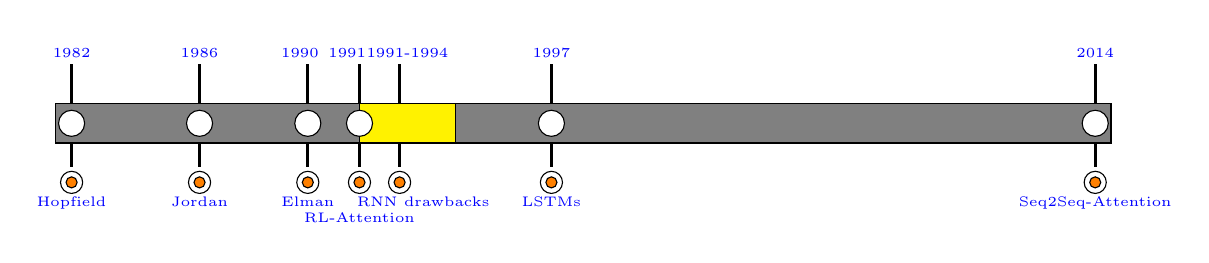
\begin{tikzpicture}[datemarker/.style={circle, draw=black,fill=white},textlabel/.style={anchor=center,text height=1.7ex,text depth=.25ex}] 
\tikzset{every node/.style={font=\tiny, color=blue}}\draw[fill=gray](-0.2,0) rectangle (13.2,0.5) node[white, below]{}; 

\onslide<2->{\node at (0.0, 0.25) [datemarker] {};}
\onslide<2->{\draw [line width=1pt] (0.0, 0.5) to (0.0, 1.0);} 
\onslide<2->{\draw (0.0, 1.2) node [textlabel] {1982 };}
\onslide<2->{\draw [fill=orange](0.0, -0.5) circle (2pt){};}
\onslide<2->{\draw (0.0, -0.5) circle (4pt){};}
\onslide<2->{\draw [line width=1pt] (0.0, 0) to (0.0, -0.3);}
\onslide<2->{\draw (0.0,-0.7) node [textlabel] {Hopfield};}

\onslide<3->{\node at (1.625, 0.25) [datemarker] {};}
\onslide<3->{\draw [line width=1pt] (1.625, 0.5) to (1.625, 1.0);} 
\onslide<3->{\draw (1.625, 1.2) node [textlabel] {1986 };}
\onslide<3->{\draw [fill=orange](1.625, -0.5) circle (2pt){};}
\onslide<3->{\draw (1.625, -0.5) circle (4pt){};}
\onslide<3->{\draw [line width=1pt] (1.625, 0) to (1.625, -0.3);}
\onslide<3->{\draw (1.625,-0.7) node [textlabel] {Jordan};}

\onslide<4->{\node at (3, 0.25) [datemarker] {};}
\onslide<4->{\draw [line width=1pt] (3, 0.5) to (3, 1.0);} 
\onslide<4->{\draw (2.9, 1.2) node [textlabel] {1990 };}
\onslide<4->{\draw [fill=orange](3, -0.5) circle (2pt){};}
\onslide<4->{\draw (3, -0.5) circle (4pt){};}
\onslide<4->{\draw [line width=1pt] (3, 0) to (3, -0.3);}
\onslide<4->{\draw (3,-0.7) node [textlabel] {Elman};}

\onslide<5->{\draw[fill=yellow](3.65625,0) rectangle (4.875,0.5){};}
\onslide<5->{\draw [line width=1pt] (4.165625, 0.5) to (4.165625, 1.0);} 
\onslide<5->{\draw (4.265625, 1.2) node [textlabel] {1991-1994 };}
\onslide<5->{\draw [fill=orange](4.165625, -0.5) circle (2pt){};}
\onslide<5->{\draw (4.165625, -0.5) circle (4pt){};}
\onslide<5->{\draw [line width=1pt] (4.165625, 0) to (4.165625, -0.3);}
\onslide<5->{\draw (4.465625,-0.7) node [textlabel] {RNN drawbacks};}


\onslide<6->{\node at (6.09375, 0.25) [datemarker] {};}
\onslide<6->{\draw [line width=1pt] (6.09375, 0.5) to (6.09375, 1.0);} 
\onslide<6->{\draw (6.09375, 1.2) node [textlabel] {1997 };}
\onslide<6->{\draw [fill=orange](6.09375, -0.5) circle (2pt){};}
\onslide<6->{\draw (6.09375, -0.5) circle (4pt){};}
\onslide<6->{\draw [line width=1pt] (6.09375, 0) to (6.09375, -0.3);}
\onslide<6->{\draw (6.09375,-0.7) node [textlabel] {LSTMs};}

\onslide<7->{\node at (13.0, 0.25) [datemarker] {};}
\onslide<7->{\draw [line width=1pt] (13.0, 0.5) to (13.0, 1.0);} 
\onslide<7->{\draw (13.0, 1.2) node [textlabel] {2014 };}
\onslide<7->{\draw [fill=orange](13.0, -0.5) circle (2pt){};}
\onslide<7->{\draw (13.0, -0.5) circle (4pt){};}
\onslide<7->{\draw [line width=1pt] (13.0, 0) to (13.0, -0.3);}
\onslide<7->{\draw (13.0,-0.7) node [textlabel] {Seq2Seq-Attention};}

\onslide<8->{\node at (3.65625, 0.25) [datemarker] {};}
\onslide<8->{\draw [line width=1pt] (3.65625, 0.5) to (3.65625, 1.0);} 
\onslide<8->{\draw (3.5, 1.2) node [textlabel] {1991 };}
\onslide<8->{\draw [fill=orange](3.65625, -0.5) circle (2pt){};}
\onslide<8->{\draw (3.65625, -0.5) circle (4pt){};}
\onslide<8->{\draw [line width=1pt] (3.65625, 0) to (3.65625, -0.3);}
\onslide<8->{\draw (3.65625,-0.9) node [textlabel] {RL-Attention};}
\end{tikzpicture}
\end{overlayarea}
\end{minipage}
\end{frame}